\chapter{Estado de la Cuestión}
\label{cap:estadoDeLaCuestion}

\section{Aplicaciones de guía}
En los últimos años ha aumentado la sensibilización tecnológica en áreas de inclusión a usuarios con discapacidad visual. De modo que las tecnologías accesibles tienen, cada vez más, un papel central en el desarrollo de aplicaciones, logrando recortar las limitaciones que antes las separaban de las personas que sufren algún tipo mayor de dificultad visual y dirigiéndose a un público más amplio.

Al igual que las personas videntes, las personas con ceguera son usuarios de aplicaciones de muy variada índole, por ello encontramos apps ya adaptadas en categorías como: redes sociales, entretenimiento, lectura, identificación de colores y objetos, etc. 

En esta sección, haremos un pequeño estudio sobre las aplicaciones accesibles existentes en el campo de la navegación, bien sea por interiores o exteriores, y su funcionamiento.
	%PRIMERA App
\subsection{Google Maps}
El pasado 10 de Octubre de 2019, en el ``World Sight Day'', Google dió a conocer la última actualización de la famosa aplicación \textit{Google Maps}\footnote{\url{https://blog.google/products/maps/better-maps-for-people-with-vision-impairments/}}. Esta incluiría una nueva característica desarrollada desde cero por y para personas con discapacidad visual que convertiría a la misma en una app accesible.

El proyecto consiste en la implementación de una nueva funcionalidad que facilita la posibilidad de recibir instrucciones de voz más detalladas y nuevos tipos de anuncios verbales muy útiles para las rutas de a pie para personas con visibilidad reducida. Algunas de las nuevas instrucciones incluidas son: informar de manera proactiva que estás en la ruta correcta, la distancia hasta el próximo giro, la dirección en la que estás caminando, avisos para cruzar con precaución si te aproximas a una gran intersección, notificaciones en caso de ser redirigido por causa de haber abandonado accidentalmente la ruta correcta, etc. De esta manera, la aplicación pretende brindar de independencia a las personas que padecen ceguera tratando de que se sientan cómodas y seguras a la hora de explorar lugares nuevos y desconocidos. La guía de voz detallada para la navegación está actualmente en desarrollo, estando ya disponible en inglés en los Estados Unidos y en japonés en Japón. Su soporte para otros idiomas y países sigue en camino.

En cuanto a la navegación por interiores, \textit{Google Maps}\footnote{\url{https://www.google.es/intl/es/maps/about/partners/indoormaps/}} con su actualización \textit{6.0} incorporó los primeros planos de ciertos edificios públicos, entre los cuales destacan aeropuertos, centros comerciales, estadios y puntos de transporte público. Gracias a esta nueva versión, \textit{Google Maps} ayuda a determinar dónde estás, en qué planta y hacia dónde ir. Para ello, basta con hacer zoom sobre un edificio cuyo plano esté disponible en la app, y este aparecerá automáticamente y completamente detallado. En la Figuras \ref{fig:ejemplo} y \ref{fig:ejemplo2} vemos un ejemplo del famoso Madison Square Garden de Nueva York.


 

\begin{figure}[t]
	\centering
	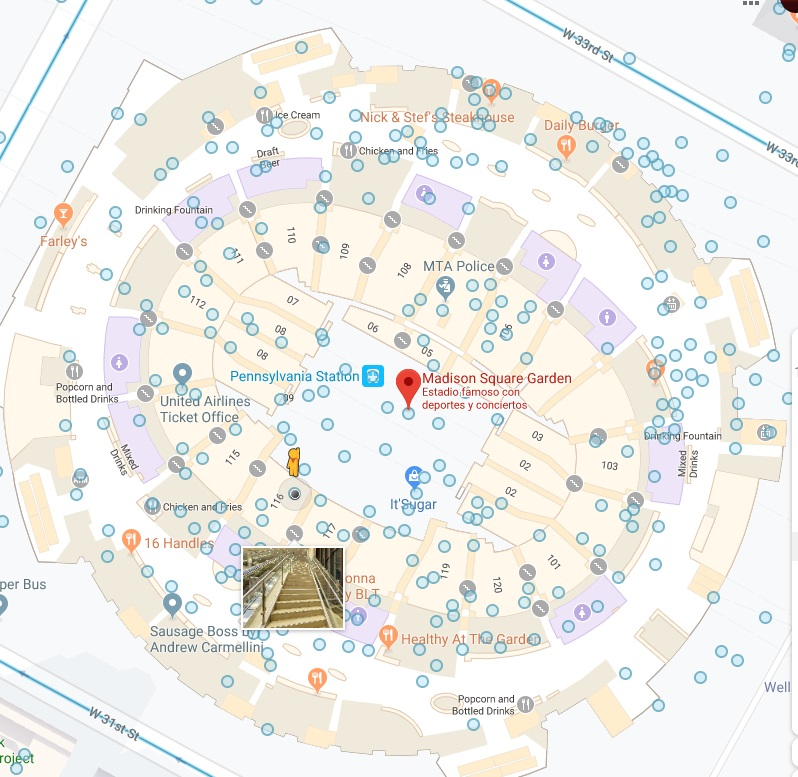
\includegraphics[width=0.6\textwidth]{Imagenes/Estadodelacuestion/MadSq2}
	\caption{Plano de un edificio proporcionado por Google Maps.}
	\label{fig:ejemplo}
\end{figure}

\begin{figure}[t]
	\centering
	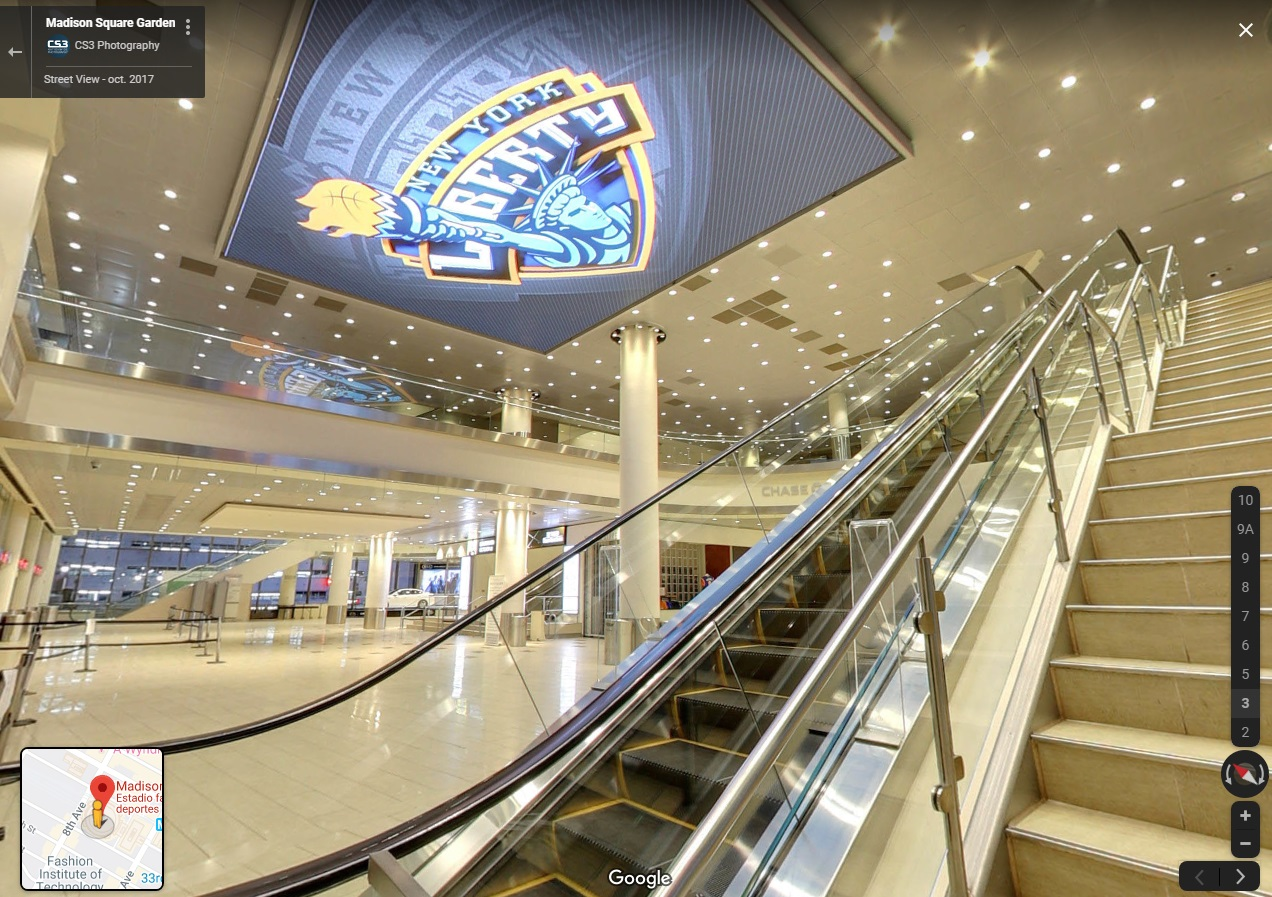
\includegraphics[width=0.6\textwidth]{Imagenes/Estadodelacuestion/MadSq3}
	\caption{Vista del interior del Madison Square Garden. }
	\label{fig:ejemplo2}
\end{figure}

Con estos nuevos planos podrás localizar dónde están los baños, escaleras, ascensores, entradas y salidas, etc., los cuales aparecen representados mediante iconos globalmente aceptados (ver Figura \ref{fig:ejemplo}). También aparecen detallados los distintos establecimientos que se localizan en el edificio e incluye la posibilidad de hacer ciertas búsquedas, tanto generales (de cafeterías, librerías, tiendas, restaurantes...) como concretas (Starbucks, McDonald's...) (ver Figura \ref{fig:ejemplo3}). Otra funcionalidad que no falta en la versión de interiores es la posibilidad de señalar un destino y recibir indicaciones sobre cómo llegar a el. Para ello, aparece el habitual punto azul que te acompaña e indica tu posición, actualizando el plano con cada movimiento que lleves a cabo (incluidos cambios de una planta a otra) (ver figura \ref{fig:ejemplo3}). Esta aplicación es un proyecto colaborativo y por ende, desde la web es posible actualizar y subir nuevos planos. Está disponible tanto para ordenador como plataformas Android e iOS.

\begin{figure}[t]
	\centering
	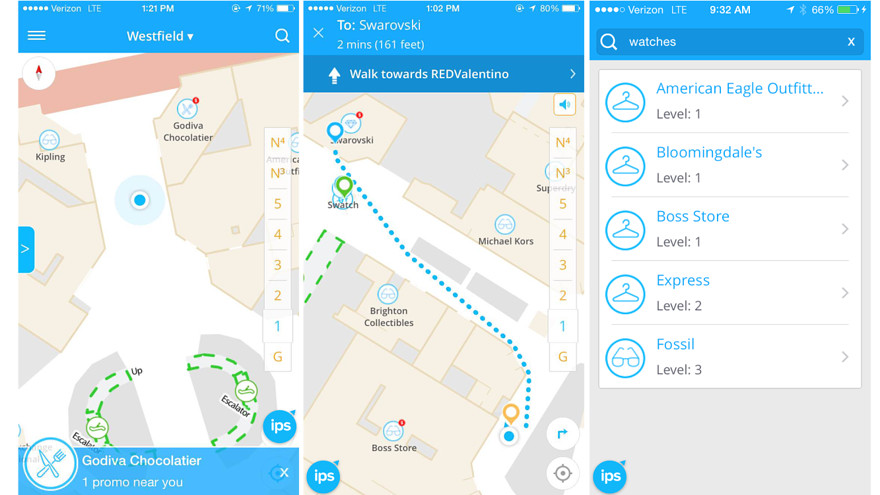
\includegraphics[width=0.6\textwidth]{Imagenes/Estadodelacuestion/GMapsInd}
	\caption{Ejemplo de navegación y búsqueda en Google Maps Indoors. }
	\label{fig:ejemplo3}
\end{figure}


Esta aplicación pone a nuestro servicio la utilidad de \textit{Maps} pero en interiores. Además, nos permite colaborar, pudiendo subir nosotros mimos el plano de un edificio. Sin dudar del gran avance que esta aplicación supone en la navegación por interiores, no debemos olvidar algunas de sus desventajas: el posicionamiento, al contrario que en exteriores, no es muy preciso (en la web hablan de varios metros), y las búsquedas que puedes realizar son limitadas, no pudiendo, por ejemplo, preguntar por la ubicación de los baños; esto es, puedes ver dónde están pero no puedes seleccionarlos como destino para que te vaya indicando la ruta a seguir. Pero sobre todo, tiene el inconveniente de que no es una tecnología accesible: \textit{Google Maps Indoors}\footnote{\url{https://www.youtube.com/watch?v=cPsTWj_O3Qs}} es una aplicación completamente visual que no cuenta con soporte auditivo por lo que descarta completamente a usuarios invidentes.



%SEGUNDA APP
\subsection{BlindSquare}
Es una de las aplicaciones de navegación más populares. Su uso se extiende a más de 130 países y está habilitada en 25 idiomas, entre los cuales se incluye el español. Esta aplicación, desarrollada para iOS y diseñada para personas con discapacidad visual, proporciona una guía completa, de origen a destino, tanto en exteriores como en interiores. Además, describe el entorno y anuncia posibles puntos de interés para el usuario (como pueden ser los lugares considerados populares o aquellos visitados frecuentemente). Su principal característica es que permite interactuar mediante voz gracias al controlador de música de Apple. 

\textit{BlindSquare}\footnote{\url{https://www.blindsquare.com}} determina tu posición mediante localización \textit{GPS} y, a partir de ahí, puede darte información sobre las proximidades utilizando \textit{Foursquare} y \textit{OpenStreetMap}. De este modo, es capaz tanto de guiarte a un cierto destino como de notificarte qué establecimientos hay en tu radio: restaurantes a 200m, parques más cercanos, farmacias...

Con el fin de agilizar el uso de la app, y que por tanto esta sea cómoda y rentable para los usuarios finales, incluye: accesos directos a funciones mediante gestos (como sacudir el móvil para que nos diga la ubicación actual y puntos cercanos) y la posibilidad de establecer filtros para recibir únicamente el tipo de información deseada. Por ejemplo, permite filtrar por restaurantes para no tener notificaciones sobre estaciones de tren o librerías.

En cuanto a la navegación por interiores, \textit{BlindSquare}\footnote{\url{https://www.youtube.com/watch?v=9jH-Bdjmgb4}} emplea un sistema de balizas bluetooth, llamadas \textit{beacons}, que colocan es sitios estratégicos de los edificios, para solventar el problema del posicionamiento. Por lo demás, incluye las mismas posibilidades y funcionalidades que la navegación por exteriores, con la única limitación de que el edificio debe estar provisto de dichos sistemas de posicionamiento.
%SOLUCIONAR VPS Y AÑADIR COMO EMPLEAN LOS BEACONS.

En su web encontramos un ejemplo de la utilización de los \textit{beacons} en un campus \footnote{\url{https://www.blindsquare.com/2019/11/01/blindsquares-getting-straight-as-on-campus/}}: una vez que entras en el edificio, uno de los \textit{beacons} se dará cuenta de tu aplicación BlindSquare y te hará saber dónde te encuentras y cómo llegar a tu destino, indicándote los ascensores, escaleras e intersecciones más cercanas. Integrar en el campus servicios como estos promueve tanto a visitantes como a estudiantes con discapacidad visual moverse por el entorno con total autonomía y seguridad.

Entre los puntos fuertes de esta aplicación destacamos los siguientes:
\begin{itemize}
	\item Da información sobre los metros que quedan hasta llegar a un determinado objetivo. Resulta útil porque si van disminuyendo sabes que vas por el camino adecuado.
	\item Utiliza indicaciones de tipo reloj (a las 10, a las 3,...) muy usadas por las personas con discapacidad visual.
	\item Avisa de las intersecciones. 
	\item Cuando te da una nueva indicación y la superas, usa el sonido asociado a correto o \textit{check}. Así, puedes seguir sin preocuparte. Si por el contrario te equivocas, reproduce un sonido en consecuencia.
	\item Se pueden añadir ubicaciones en una lista de lugares marcados.
	\item Puedes ir girando con el móvil y te va indicando lo que tienes enfrente. 
	\item También tiene opción de simulación, que permite prepararse un camino antes de ir.
	\item Te permite ser más autónomo y descubrir nuevos sitios.
	\item A la hora de desplazarte te indica las distintas alternativas por adelantado. Esto es, mientras que para espacios exteriores te señala la posible ruta utilizando transporte público, privado, a pie, etc. Para espacios interiores te especifica, siempre que la haya, la opción de utilizar escaleras, ascensor, escaleras mecánicas, etc., de esta manera te proporciona una idea global del espacio y de las distintas vías que puedes seguir para llegar a tu destino.
	\item Permite llevar las manos libres.
	\item Incluye un lector de códigos QR, es más cómodo porque puede dar más información que la línea braille.
\end{itemize}

Su principal punto negativo es el precio, ya que cuesta 40 libras.

Al contrario que la aplicación anterior, esta sí es una aplicación diseñada para personas con discapacidad visual. Las diferencias saltan a la vista: el modo de dar las indicaciones, avisos constantes para indicarte si vas por el camino correcto, permite más autonomía; gracias a la comunicación constante que ofrece permite llevar las manos libres, entre otras. Parece imposible pensar que el interior de un edificio pueda resultar menos seguro que una gran avenida, lo cierto es, que para personas con discapacidad visual, muchas veces es así. El interior de un gran centro comercial o una biblioteca resultan un laberinto cuando se va por primera vez, más aún si tenemos algún tipo de dificultad para leer las indicaciones que, normalmente, suelen estar en lugares altos y no adaptadas para personas con discapacidad visual. Lo que se pretende con esta aplicación es mantener la autonomía del usuario tanto dentro como fuera de un edificio \footnote{\url{https://www.blindsquare.com/2019/10/24/independence-on-both-sides-of-the-door/}}.


%CONCLUSIÓN DE POR QUÉ TODO ESTO ES BUENO PARA LOS CIEGOS.

\subsection{Nearby Explorer}
\textit{Nearby Explorer}\footnote{\url{https://play.google.com/store/apps/details?id=org.aph.nearbyonline&hl=es}} es otra de las aplicaciones que encuadramos en el campo de la navegación accesible por interiores y exteriores. Está habilitada tanto para Android como para iOS y su descarga se encuentra disponible en el \textit{App Store} de manera gratuita. 

La guía por exteriores se basa en la misma idea que \textit{BlindSquare}, y por ende funciona de manera similar. Entre sus características destacan: la posibilidad de ejecutar ciertas acciones poniendo el móvil en distintas posiciones, como por ejemplo, inclinarlo verticalmente para que funcione como una brújula; y, la capacidad de filtrar la información de modo que ésta se adapte completamente a las necesidades del usuario. Entre la información que \textit{Nearby Explorer} puede proporcionar a sus usuarios encontramos los lugares cercanos a la ubicación actual, los nombres de las calles por las que pasa, los números de los bloques de las calles por las que pasa, la distancia que hay al destino desde un punto de referencia (como casa, trabajo...), etc. Además de la posibilidad de filtrar la información deseada, las indicaciones por audio pueden ser pausadas en cualquier momento de modo que no interfieran con otras señales auditivas (como las paradas en un autobús, por ejemplo). Otra gran funcionalidad con la que cuenta \textit{Nearby Explorer} es la de explorar una ruta por adelantado, sin tener que estar físicamente en el sitio, pudiendo incrementar o decrementar el radio de exploración.

Por otro lado, vemos que la navegación por interiores puede ser configurada de dos maneras: \textit{ad hoc} y \textit{mapeo completo}. Ambas utilizan los sistemas de \textit{beacons} para geolocalizar el dispositivo en interiores (zonas a las que no llega el \textit{GPS}) y así, poder proprocionar una guía por dicho espacio.

En el caso de la configuración \textit{ad hoc} aparecen los siguientes problemas:
\begin{itemize}
	\item No se puede determinar la ubicación de un \textit{beacon}.
	\item No se puede obtener información del entorno a menos que te encuentres dentro del radio de detección de un \textit{beacon}.
	\item Tienes que habilitar cierto soporte para detectar los \textit{beacons} (no se detectan de manera automática).
\end{itemize}

Sin embargo, el \textit{mapeo completo} sí nos proporciona una localización precisa. Tiene un comportamiento similar al de otras aplicaciones.

%REFLEXIÓN

\subsection{Lazarillo}
Lazarillo \citep{lazarilloOnline} es una aplicación que actualmente solo proporciona guía para exteriores. Inicialmente la idea era cubrir también la navegación por interiores pero su desarrollo no fue posible por problemas de financiación.

La navegación por exteriores cuenta con las funcionalidades básicas que ya hemos mencionado en las apps anteriores: \begin{itemize}
	\item Buscar lugares de interés, cercanos a la ubicación actual. Esta búsqueda se puede acotar filtrando por categorías que vienen predefinidas (transporte, bancos y cajeros, salud, comida, tiendas, etc.).
	\item Buscar una dirección específica a partir de la cual se desplegarán todas las posibles rutas (a pie, en transporte público, privado, etc.) y una vez seleccionada la ruta deseada, comenzarán las indicaciones mediante audio con la información pertinente (metros, giros a derecha e izquierda, etc. ). 
	\item Guardar una lista de lugares favoritos.
	\item Posibilidad de rastrear una dirección, previamente marcada con la opción ``Seguir este lugar'', de modo que con independencia de a dónde nos estemos dirigiendo se activará una alerta a medida que nos acerquemos a dicha ubicación.
	\item Ajustar la configuración de las indicaciones, velocidad, tipo de voz...
\end{itemize}

En resumidas cuentas, \textit{Lazarillo} es una aplicación que, como otras, busca mejorar la calidad de vida de las personas con discapacidad visual indicándoles para ello qué les rodea y proporcionándoles una mayor independencia. Ésta, sin embargo, cubre únicamente los aspectos más básicos y elementales, sin reparar en otras posibles funcionalidades o indicaciones (obstáculos, peligros...) que la convierten en una aplicación incompleta.

La app es completamente gratuita y cuenta con versión para Android y iOs.
\subsection{Wayfindr} 
Wayfindr \citep{wayfindrOnline} es una aplicación cuyo objetivo es guiar a los invidentes por el metro de Londres (uno de los más complejos del mundo). Este proyecto, aún no disponible para el público, pretende llegar a esos lugares que están repletos de señales escritas, por los que las personas que ven pasan sin pensar pero que son precisamente los que más temen y evitan aquellos que tienen discapacidad visual. Investigaciones llevadas a cabo en el Reino Unido revelan que la mayor parte de este colectivo querría salir de su hogar con más frecuencia. Por ello, la sociedad británica \textit{Royal Society for Blind Children (RSBC)} y \textit{UsTwoo}, plataforma de innovación y tecnología digital, se unieron para desarrollar una solución, naciendo así, Wayfindr.

El funcionamiento\footnote{\url{https://www.youtube.com/watch?v=mc3KmbfxuUQ}} de la aplicación es tan práctico como sencillo: se basa en una serie de \textit{beacons}, colocados en puntos estratégicos a lo largo de las distintas estaciones de metro, que emiten unas señales que son captadas por el móvil a su paso por un cierto radio de detección. Estas señales permiten ubicar al usuario y darle la siguiente indicación para el conseguimiento de su objetivo (coger un tren o salir de la estación).

Los desarrolladores recomiendan el uso de auriculares de conducción ósea, de manera que puedan escuchar otros sonidos del exterior.

\subsection{Conclusiones}
Tras este breve recorrido por algunas de las aplicaciones de navegación adaptadas para personas ciegas o con visibilidad reducida podemos decir que cada vez son más las opciones. Hemos visto desde aplicaciones de navegación por exteriores, como también por interiores, llegando hasta algunas tan específicas como \textit{Wayfindr} que está dirigida al metro de Londres concretamente. Todas ellas se rigen por un patrón común: el de la simpleza, sin conllevar por ello una reducción de la funcionalidad. Pues estas aplicaciones nos permiten filtrar la información que se quiere recibir, guardar nuestros lugares más visitados, manejarlas mediante voz o con sacudidas del teléfono..., es decir, nos proporcionan un gran abanico de posibilidades que el usuario puede ejecutar de manera sencilla.

Por otro lado, si comparamos las apps, encontramos que aquellas de navegación por interiores están aún por desarrollar ya que el mapeo del interior de los edificios debe realizarse de manera particular e individual, convirtiéndose en una tarea mucho más tediosa que la que lleva a cabo el famoso coche de \textit{Google Maps}. Además, el posicionamiento también es más complejo ya que no es posible utilizar el sistema GPS y hay que recurrir a la triangulación de señales WIFI o a las balizas bluetooth, teniendo que estudiar de nuevo cada caso concreto.


\section{Sistemas de posicionamiento}
Para la consecución de nuestro objetivo, el desarrollo de una aplicación de navegación por interiores, uno de los primeros problemas que se nos plantea es el del posicionamiento en un mapa ya que es de vital importancia poder determinar donde estamos para después indicar la ruta pertinente hacia el destino indicado. En esta sección haremos un pequeño estudio sobre las distintas tecnologías existentes que nos permiten solventar nuestro problema y determinar la posición exacta de un cierto dispositivo, y discutiremos su validez para la consecución del objetivo de este trabajo de fin de grado.

\subsection{GPS}

El Sistema de Posicionamiento Global (GPS) es un sistema de localización, diseñado por el Departamento de
Defensa de los Estados Unidos con fines militares para proporcionar estimaciones precisas de posición,
velocidad y tiempo. Este sistema se encuentra operativo desde enero de 1994 y se desarrolló a partir de los 24 satélites que componen la constelación NAVSTAR, cada uno de los cuales cuenta con una órbita de 26560Km de radio y un periodo de 12h \citep{pozo2000sistema}. 

El método mediante el cual el GPS determina la altitud, longitud y latitud de cualquier objeto que se encuentre en la superficie terrestre se conoce como triangulación. Este requiere la distancia desde el dispositivo en cuestión (receptor) a tres satélites como mínimo cuya localización es conocida de antemano. Entonces, cuando el receptor detecta el primer satélite, se genera una esfera a su alrededor cuyo radio será la distancia desde el receptor hasta dicho satélite. De este modo, el receptor se encontrará en un punto de la superficie de esa esfera, aún por determinar. Repetimos el proceso con otro satélite. Al crearse esa segunda esfera, el dispositivo receptor se encontrará en alguno de los puntos de corte de ambas esferas, por lo que el resto de puntos se descartan. De nuevo, se utiliza un tercer satélite de modo que se crea una nueva esfera que cortará a las
anteriores. De este modo, con el corte de las tres esferas, y teniendo en cuenta que el dispositivo se encuentra en la superficie terrestre, tendremos el punto concreto buscado. En caso de querer conocer la altitud, bastará con usar un cuarto satélite como referencia y repetir el proceso. En la Figura \ref{fig:ejemplogps} vemos un esquema del proceso que acabamos de explicar empleando 3 y 4 satélites.

El problema del Sistema de posicionamiento Global es que pierde mucha precisión cuando nos encontramos bajo superficies como túneles, tejados, etc. ya que la señal se debilita enormemente y el dispositivo no es capaz de llevar a cabo la triangulación de manera exacta. Es por esto, que descartamos este sistema para nuestro propósito.

\begin{figure}[t]
	\centering
	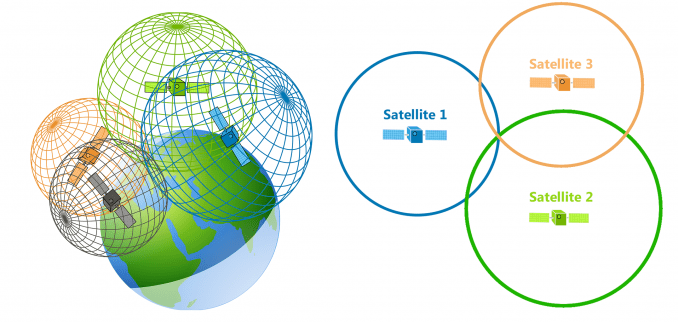
\includegraphics[width=0.6\textwidth]{Imagenes/Estadodelacuestion/triangulacion}
	\caption{Método de triangulación GPS. }
	\label{fig:ejemplogps}
\end{figure}


\subsection{Wi-Fi}
 %Esta técnica se basa en leer con un dispositivo la intensidad de señal que recibe de distintos puntos de acceso Wi-Fi del edificio y triangularla para determinar la posición exacta.

\subsection{Balizas Bluetooth}

Los \textit{beacons} o balizas bluetooth son pequeños dispositivos que emiten señales de radio. Estas señales los identifican de manera única y pueden ser captadas por otros dispositivos receptores, estableciéndose así un canal de comunicación que permanece vivo siempre que permanezcan en un radio de alcance de entre 10 y 30 metros como máximo, según el dispositivo. Es importante remarcar que generalmente los \textit{beacons} no aceptan conexiones de otros dispositivos, lo que significa que no pueden registrar qué aparatos están cerca. Por tanto, esta simplicidad conlleva la necesidad de una aplicación capaz de interpretar la señal de la baliza. Otra característica de los \textit{beacons} es que son de bajo consumo, es decir, sus baterías tienen una duración muy prolongada (aproximadamente 2 años) con una simple pila de botón, y su coste es reducido.

Esta tecnología se hizo muy popular en 2013 cuando Apple introdujo el \textit{iBeacon} estándar y comenzó a utilizarlos para la navegación, más concretamente, para el posicionamiento en interiores. En 2015 Google, que no quiso quedarse atrás, lanzó el protocolo Eddystone, un protocolo, que a diferencia del de Apple, es de código abierto y ofrece soporte oficial tanto para iOS como para Android. Otras de las ventajas que incluye la versión de Google es que proporciona dos APIs que facilitan mucho el manejo de los \textit{beacons} y que emite 4 paquetes distintos de información, en lugar de 1 como en el caso de los iBeacons. Estos paquetes son:

\begin{itemize}
	\item \textbf{Eddystone-UID:} transmite un identificador de baliza único compuesto por 16 bytes, 10 de ellos referidos al espacio de nombres, que identifican a un grupo de \textit{beacons}, y 6 que se refieren e identifican a la instancia particular dentro del grupo. Esta distinción entre espacio de nombres e instancia se pensó para optimizar el escaneo de beacons. Este paquete es idéntico al que ofrecen los \textit{iBeacons}.
	\item \textbf{Eddystone-URL:} transmite una URL utilizando un formato de codificación.
	\item \textbf{Eddystone-TLM:} transmite información sobre la baliza. Como puede ser el nivel de la batería, los datos del sensor u otra información relevante para los administradores de balizas. Para poder usarse también como baliza necesita ir acompañado de otro tipo de marco (Eddystone-URL o Eddystone-UID).
	\item \textbf{Eddystone-EID:} emite un identificador encriptado que cambia periódicamente, de modo que su uso está restringido a aplicaciones y dispositivos autorizados.
\end{itemize}

Por todo esto, consideramos que el protocolo Eddystone es más ventajoso.
 %SEGUIR PENSANDO COMO PONER LA CONCLUSIÓN DE QUE USAMOS BEACONS.
Para el motivo de nuestro estudio, la navegación por interiores, esta tecnología bluetooth es muy útil: basta con colocar las balizas en puntos de interés (\textit{landmarks}) del edificio en cuestión y tener una aplicación que interprete las señales que recibe para saber donde se encuentra exactamente el usuario. No obstante, hay que tener en cuenta que la disposición exacta de los \textit{beacons} y la cantidad necesaria para mapear un área dependerá del edificio concreto.

Aunque la alternativa tecnológica Wi-Fi es también adecuada para solventar el problema del posicionamiento en interiores y cuenta con ventajas como la de aprovechar la infraestructura del edificio, también conlleva inconvenientes como que el posicionamiento basado en cliente-servidor no está soportado en dispositivos Apple, por lo que usando Wi-Fi estaríamos descartando a una gran catidad de los potenciales usuarios que cuenten con un dispositivo móvil iOS. Además entre las ventajas que nos ofrecen los \textit{beacons} destaca su flexibilidad: podemos colocarlos donde queramos, son pequeños y ligeros y proporcionan una exactitud de 1 a 3 metros, frente a una de 5 a 15 con la señal Wi-Fi. 

%NO ENTIENDO NADA DE ESTO:
%La navegación por interiores no es el único uso que se le puede dar a los beacons. Con ellos podemos, por ejemplo, traquear de dispositivos en una oficina (como proyectores o portátiles), dar a conocer un establecimiento (la instalación de un beacon puede hacerlo más accesible, una persona ciega puede reconocer el establecimiento gracias a la señal que ha captado su móvil), el análisis de los flujos de personas en centros públicos como aeropuertos, entre otras. 




 